%%%%%%%%%%%%%%%%%%%%%%%%%%%%%%%%%%%%%%%%%
% Short Sectioned Assignment LaTeX Template Version 1.0 (5/5/12)
% This template has been downloaded from: http://www.LaTeXTemplates.com
% Original author:  Frits Wenneker (http://www.howtotex.com)
% License: CC BY-NC-SA 3.0 (http://creativecommons.org/licenses/by-nc-sa/3.0/)
%%%%%%%%%%%%%%%%%%%%%%%%%%%%%%%%%%%%%%%%%

%----------------------------------------------------------------------------------------
%	PACKAGES AND OTHER DOCUMENT CONFIGURATIONS
%----------------------------------------------------------------------------------------

\documentclass[paper=a4, fontsize=11pt]{scrartcl} % A4 paper and 11pt font size

% ---- Entrada y salida de texto -----

\usepackage[T1]{fontenc} % Use 8-bit encoding that has 256 glyphs
\usepackage[utf8]{inputenc}
%\usepackage{fourier} % Use the Adobe Utopia font for the document - comment this line to return to the LaTeX default

% ---- Idioma --------

\usepackage[spanish, es-tabla]{babel} % Selecciona el español para palabras introducidas automáticamente, p.ej. "septiembre" en la fecha y especifica que se use la palabra Tabla en vez de Cuadro

% ---- Otros paquetes ----

\usepackage{url} % ,href} %para incluir URLs e hipervínculos dentro del texto (aunque hay que instalar href)
\usepackage{hyperref}
\hypersetup{
	colorlinks=true,
	linkcolor=black,
	urlcolor=black,
	citecolor=black,
}
\usepackage{amsmath,amsfonts,amsthm} % Math packages
%\usepackage{graphics,graphicx, floatrow} %para incluir imágenes y notas en las imágenes
\usepackage{graphics,graphicx, float} %para incluir imágenes y colocarlas

% Para hacer tablas comlejas
%\usepackage{multirow}
%\usepackage{threeparttable}

%\usepackage{sectsty} % Allows customizing section commands
%\allsectionsfont{\centering \normalfont\scshape} % Make all sections centered, the default font and small caps

\usepackage{fancyhdr} % Custom headers and footers
\pagestyle{fancyplain} % Makes all pages in the document conform to the custom headers and footers
\fancyhead{} % No page header - if you want one, create it in the same way as the footers below
\fancyfoot[L]{} % Empty left footer
\fancyfoot[C]{} % Empty center footer
\fancyfoot[R]{\thepage} % Page numbering for right footer
\renewcommand{\headrulewidth}{0pt} % Remove header underlines
\renewcommand{\footrulewidth}{0pt} % Remove footer underlines
\setlength{\headheight}{13.6pt} % Customize the height of the header

\numberwithin{equation}{section} % Number equations within sections (i.e. 1.1, 1.2, 2.1, 2.2 instead of 1, 2, 3, 4)
\numberwithin{figure}{section} % Number figures within sections (i.e. 1.1, 1.2, 2.1, 2.2 instead of 1, 2, 3, 4)
\numberwithin{table}{section} % Number tables within sections (i.e. 1.1, 1.2, 2.1, 2.2 instead of 1, 2, 3, 4)

\setlength\parindent{0pt} % Removes all indentation from paragraphs - comment this line for an assignment with lots of text

\newcommand{\horrule}[1]{\rule{\linewidth}{#1}} % Create horizontal rule command with 1 argument of height

\usepackage{listings}
\usepackage{color}
\usepackage{xcolor}
\lstdefinestyle{customc}{
	belowcaptionskip=1\baselineskip,
	breaklines=true,
	frame=L,
	xleftmargin=\parindent,
	language=C,
	showstringspaces=false,
	basicstyle=\footnotesize\ttfamily,
	keywordstyle=\bfseries\color{green!40!black},
	commentstyle=\itshape\color{purple!40!black},
	identifierstyle=\color{blue},
	stringstyle=\color{orange},
}

\lstset{escapechar=@,style=customc}

\title{	
	\normalfont \normalsize 
	\textsc{\textbf{Inteligencia de Negocio} \\ Grado en Ingeniería Informática \\ Universidad de Granada \\
	Curso 2017-2018} \\ [25pt] % Your university, school and/or department name(s)
	\horrule{0.5pt} \\[0.4cm] % Thin top horizontal rule
	\huge Memoria Práctica 2. \\
	\huge Clustering.
	\\ % The assignment title
	\horrule{2pt} \\[0.5cm] % Thick bottom horizontal rule
}

\author{Alberto Armijo  \\
\href{mailto:armijoalb@correo.ugr.es}{armijoalb@correo.ugr.es}} % Nombre y apellidos
\date{\normalsize\today} % Incluye la fecha actual

%----------------------------------------------------------------------------------------
% DOCUMENTO
%----------------------------------------------------------------------------------------

\begin{document}
	
	\maketitle % Muestra el Título
	
	\newpage %inserta un salto de página
	
	\tableofcontents % para generar el índice de contenidos
	
	\listoffigures % para generar índice de imágenes.
	
	\listoftables % para generar índice de tablas.
	
	\newpage
	
	\section[Introducción]{Introducción.}
	En esta práctica se desarrollará un estudio para ver similaridades y relaciones de causalidad para explicar tipos y gravedad de accidentes de tráfico.
	
	\vspace{0.06in}
	Para el estudio de los datos, se utilizará una base de datos sobre accidentes publicada por la Dirección General de Tráfico (DGT). Dentro de esta base de datos se pueden encontrar 30 variables diferentes, entre las cuáles se encuentran el número de heridos, tanto leves como graves, el número de muertos, el número de vehículos implicados en el accidente, la localidad donde se ha producido el accidente, el tipo de accidente que ha sido, etc...
	
	\vspace{0.06in}
	Para realizar este estudio, se usarán 5 algoritmos de clustering diferentes, para los cuáles se analizarán varias métricas y gráficas para analizar los resultados obtenidos.
	\section[Casos de estudio]{Casos de estudio.}
	Dentro de este apartado, se realizarán 3 casos de estudio, en cada uno de ellos se ejecutarán los algoritmos de clustering seleccionados. Después se calcularán las métricas, gráficas para su posterior análisis.
	
	Los algoritmos de clustering que se utilizará para el estudio son:
	\begin{itemize}
		\item K-medias.
		\item Agglomerative Clustering.
		\item Mean Shift.
		\item Birch.
		\item Spectral Clustering.
	\end{itemize}

	Las métricas que se utilizarán para comparar los datos son: número de clusters, índice Calinski-Harabaz, la métrica Silhouette y el tiempo de ejecución de cada algoritmo.
	
	\vspace{0.06in}
	Dentro de nuestro conjunto de datos, tenemos las siguientes variables:
	\begin{itemize}
		\item \textbf{Numéricas:}
			\subitem Mes en el que ocurrió el accidente. Numerados del 1 al 12.
			\subitem Hora del accidente. Numerados del 0 al 23.
			\subitem Día de la semana. Numerados del 1 al 7.
			\subitem Total de víctimas \textbf{(TOT\_VICTIMAS)}. Representa el número de víctimas implicadas en el accidente.
			\subitem Total de víctimas durante 30 días. \textbf{(TOT\_VICTIMAS30D)}. Representa la media de la víctimas implicadas durante el mes.
			\subitem Total de muertos (\textbf{TOT\_MUERTOS)}. Representa el número de muertos que ha habido en el accidente.
			\subitem Total de muertos durante 30 días \textbf{(TOT\_MUERTOS30D)}. Representa la media de muertos que ha habido durante 30 días.
			\subitem Total de heridos graves. \textbf{(TOT\_HERIDOS\_GRAVES)} Representa el número de heridos graves en el accidente.
			\subitem Total de heridos graves durante 30 días. \textbf{(TOT\_HERIDOS\_GRAVES30D)} Representa la media de heridos graves durante 30 días.
			\subitem Total de heridos leves. \textbf{(TOT\_HERIDOS\_LEVES)} Representa el número de heridos leves implicados en el accidente.
			\subitem Total de heridos leves durante 30 días. \textbf{(TOT\_HERIDOS\_LEVES30D)} Representa la media de heridos leves implicados durante 30 días.
			\subitem Total de vehículos implicados. \textbf{(TOT\_VEHICULOS\_IMPLICADOS)} Representa el número de vehículos implicados en el accidente.
		
		
		\item \textbf{No numéricas:}
		\subitem \textbf{Provincia}. Provincia donde se produjo el accidente.
		\subitem \textbf{Comunidad Autónoma}. Comunidad Autónoma donde se produjo el accidente.
		\subitem \textbf{Isla}. Indica si la isla en la que se ha producido el accidente, si se produce dentro de la península, su valor es NO\_ISLA.
		\subitem \textbf{Zona}. Indica si se ha producido en una carretera o en una variante.
		\subitem \textbf{Zona agrupada}. Indica el tipo de vía en el que se ha producido el accidente (interurbanas o urbanas).
		\subitem \textbf{Red de carretera}. Indica el tipo de carretera en el que se ha producido el accidente (municipal, estatal,...).
		\subitem \textbf{Tipo vía}. Indica el tipo de vía en el que se ha producido el accidente (autovía, vía convencional,...).
		\subitem \textbf{Trazado o interesección.} Indica si el lugar del accidente es una recta, una intersección, o una curva.
		\subitem \textbf{Tipo de intersección.} Indica el tipo de intersección en el que se produjo el accidente. Si no es una intersección su valor es NO\_ES\_INTERSECCIÓN.
		\subitem \textbf{Acondicionamiento de la calzada}. Indica las condiciones de la calzada en la que se ha producido el accidente.
		\subitem \textbf{Prioridad}. Indica si existe algún tipo de prioridad para los vehículos (semáforo, stop, ninguna,...).
		\subitem \textbf{Superficie mojada}. Indica si la superficie la calzada está mojada, seca, si tiene aceite, o si es de otro tipo.
		\subitem \textbf{Luminosidad}. Indica la luminosidad que había cuando se produjo el accidente, si era de día, de noche, de noche sin iluminación, etc...
		\subitem \textbf{Factores atmosféricos.} Indica si había algún factor atmosférico cuando se produjo el accidente. Si estaba lloviendo, si había viento, etc...
		\subitem \textbf{Visibilidad}. Indica el tipo de visibilidad que había cuando se produjo el accidente; poca provocada por la lluvia, otra causa,...
		\subitem \textbf{Otra causa}. Indica otras causas por la que se produjo el accidente.
		\subitem \textbf{Aceras}. Indica si había aceras donde se produjo el accidente.
		\subitem \textbf{Tipo de accidente}. Indica el tipo de accidente que se ha producido; si ha habido colisión de vehículos ( y el tipo de esta colisión), vuelco en la calzada, otro tipo, ...
		\subitem \textbf{Densidad de circulación}. Indica la densidad de tráfico que había cuando se produjo el accidente.
		\subitem \textbf{Medidad especiales}. Indica si se ha tomado alguna medida especial para el accidente.
	\end{itemize}

	
	\subsection[Caso de estudio 1]{Primer caso de estudio: accidentes de colisión de vehículos en islas.}
	\subsubsection{Introducción.}
	Para este primer caso de estudio, estudiaremos aquellos accidentes en los cuáles hay colisión entre vehículos en alguna de las islas (Gran Canaria, Lanzarote, Mayorca).
	
	\vspace{0.06in}
	Las variables que vamos a utilizar son el total de vehículos implicados, total de heridos leves, total de heridos graves, total de muertos y total de victimas. El tamaño de la muestra es de 5782, por lo que utilizaremos toda la muestra para hacer el estudio. 
	
	\vspace{0.06in}
	
	\subsubsection{Parámetros de los algoritmos.}
	Para este primer caso de estudio, utilizaremos un número de clusters igual a 4 para los algoritmos de Spectral Clustering y K-Medias. Para el algoritmo Birch se ha utilizado un número de clusters igual a 6. Para el algoritmo de Mean Shift no se necesita definir el número de clusters, pero sí que necesitamos definir el parámetro bandwidth; para ello utilizaremos la función estimate\_bandwidth() indicándole como parámetros quantile=0.2 y random\_state=123456.Por último, al algoritmo Agglomerative Clustering le indicaremos que el número de clusters a de ser 38, el método que tiene que utilizar para calcular la jerarquía ha de ser \textit{ward}.
	
	\vspace{0.06in}
	
	En la tabla mostrada se verá que el número de clusters utilizados en el algoritmo de Agglomerative Clustering es siempre igual al del algoritmo Mean Shift; esto es así porque me dí cuenta de que el algoritmo de Agglomerative Clustering obtenía bastante buenos resultados utilizando el mismo tamaño de cluster.
	
	\subsubsection{Resultados obtenidos.} 
	
	\begin{table}[H]
	\centering
		\begin{tabular}{lrrrr}
			\toprule
			Name &      HC metric &  SC metric &      Time(s) &  N Clusters \\
			\midrule
			AC         &  168372.5444 &   0.9743 &  0.4195 &          38 \\
			Mean Shift &   12602.8918 &   0.9063 &  0.0796 &          38 \\
			SpectralC  &   10108.4158 &   0.8073 &  3.5854 &           4 \\
			Birch      &    7283.9452 &   0.8039 &  0.0799 &           6 \\
			K-medias   &   11042.6260 &   0.8311 &  0.0234 &           4 \\
			\bottomrule
		\end{tabular}
	\caption{Resultados algoritmos en el primer caso de estudio}
	\label{table:res_caso1}
	\end{table}

	Para este caso de estudio el algoritmo que mejor resultados obtiene es el Agglomerative Clustering, dado que ambas métricas tienen los valores más altos. Compararemos este algoritmo con el K-Medias, que con un número menor de clusters obtiene también buenos resultados.

	\subsubsection{Interpretación de la segmentación.}
	Para interpretar los resultados obtenidos por cada uno de los algoritmos, vamos a utilizar un scatter matrix y un heatmap por cada uno de ellos. En heatmap contendrá como filas los clusters y como columnas, obtendremos la media de los valores de esa variable en ese cluster.
	
	\vspace{0.06in}
	
	Primero utilizaremos los heatmap ya que nos dan de una forma más rápida de entender de forma más general cuáles son las características que utilizan los distintos clusters. Después utilizaremos los scatter matrix para intentar obtener más detalle.
	
	\begin{figure}[H]
		\centering
		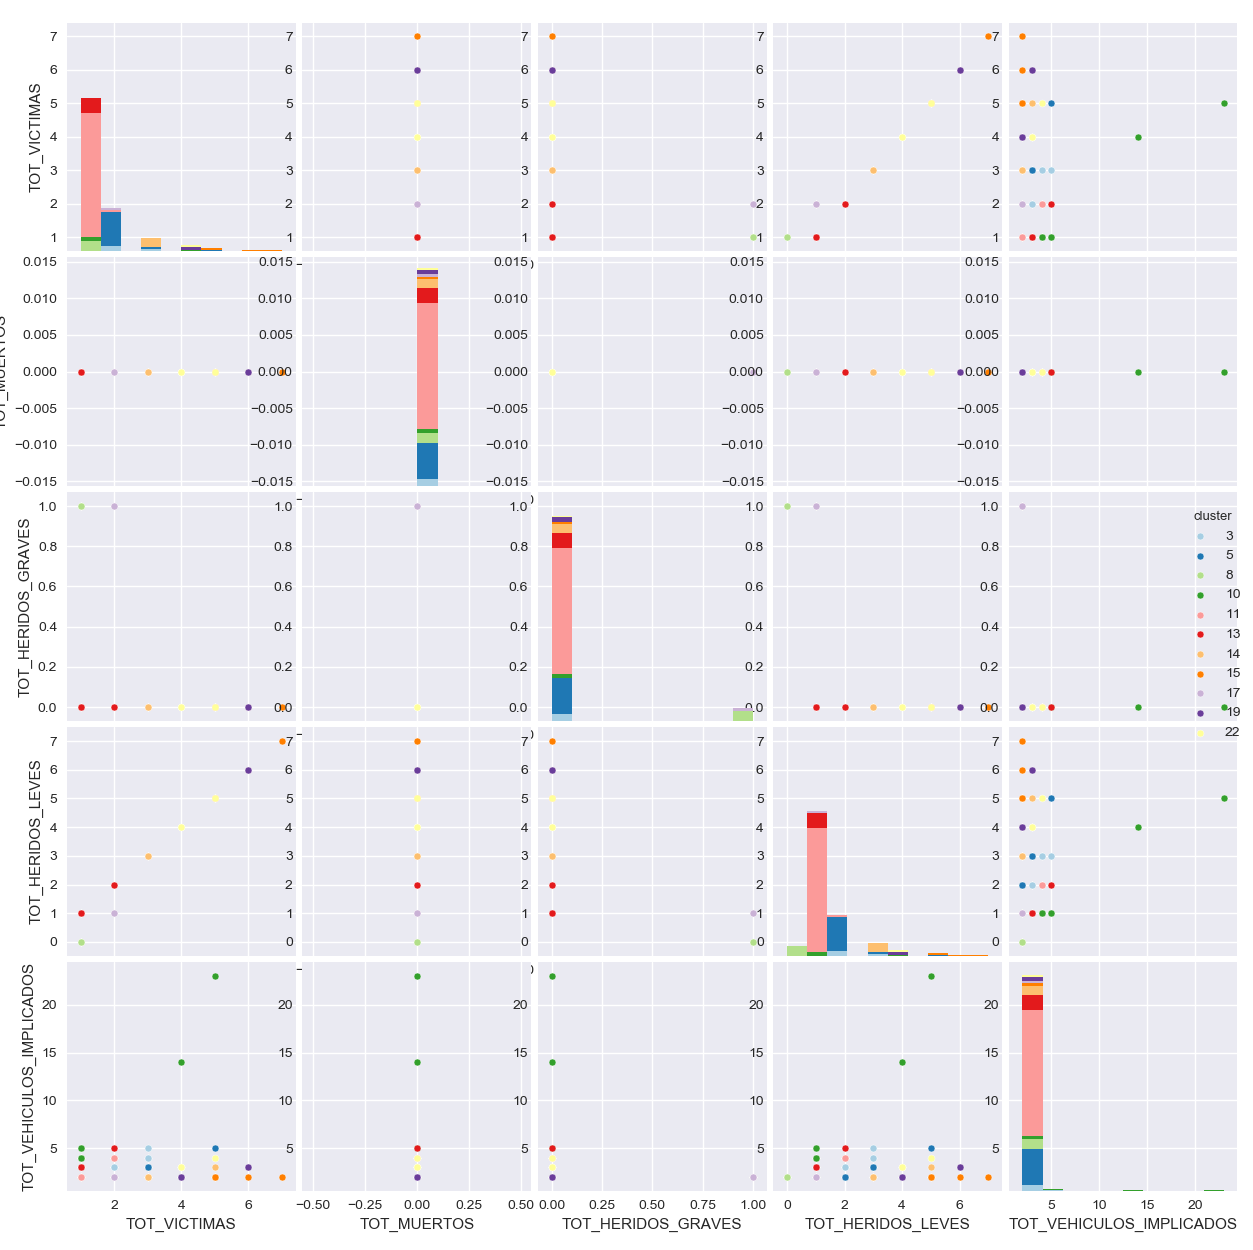
\includegraphics[scale=0.25]{../imagenes/scatterMatrix_caso1_AC.png}
		\caption{Scatter Matrix Agglomerative Clustering}
		\label{fig:scatter_caso1_AC}
	\end{figure}

	\begin{figure}[H]
		\centering
		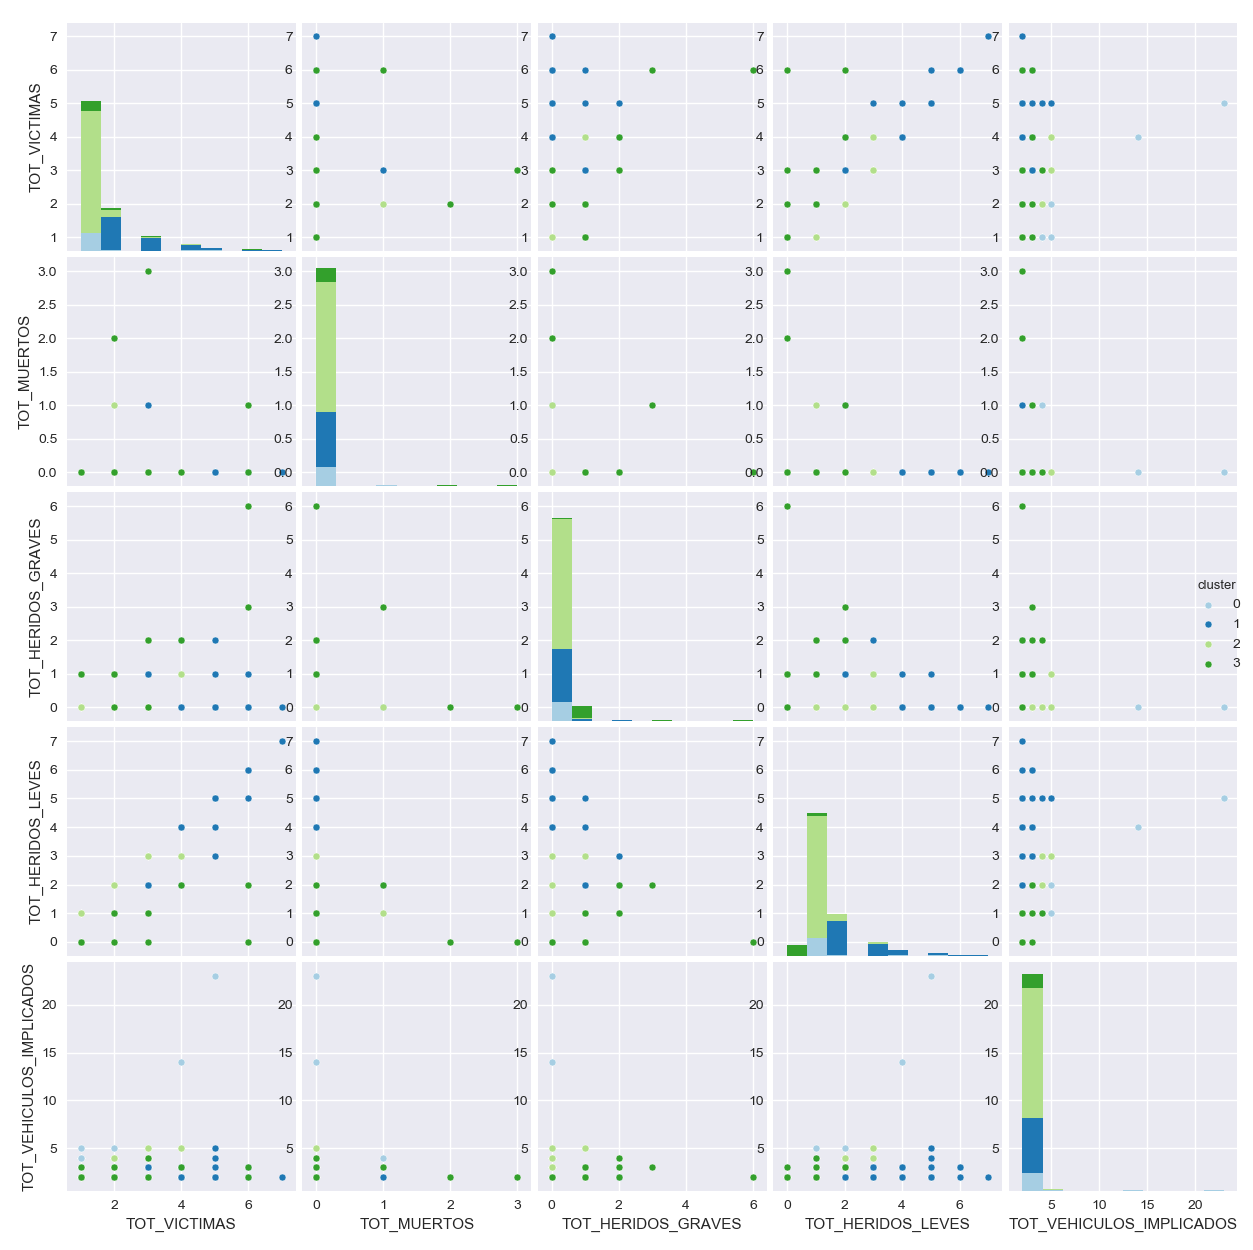
\includegraphics[scale=0.25]{../imagenes/scatterMatrix_caso1_K-medias.png}
		\caption{Scatter Matrix KMedias}
		\label{fig:scatter_caso1_KMedias}
	\end{figure}

	\begin{figure}[H]
		\centering
		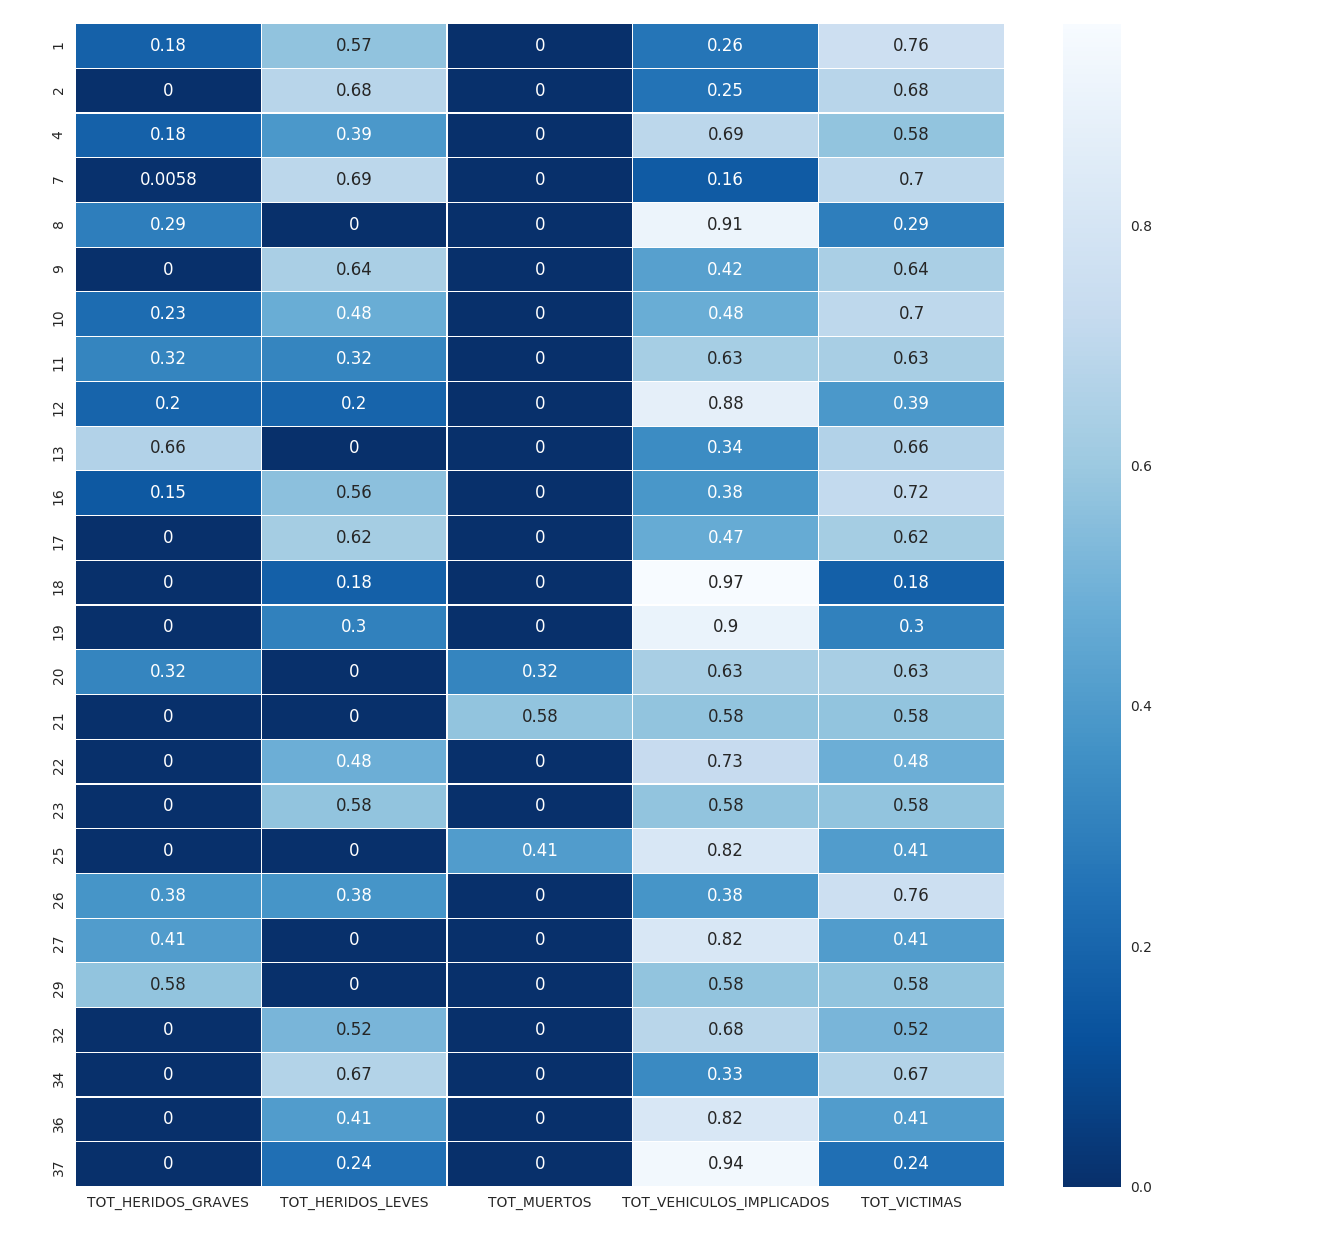
\includegraphics[scale=0.3]{../imagenes/heatmap_caso1_AC.png}
		\caption{Heatmap Agglomerative Clustering}
		\label{fig:hm_caso1_AC}
	\end{figure}
	
	\begin{figure}[H]
		\centering
		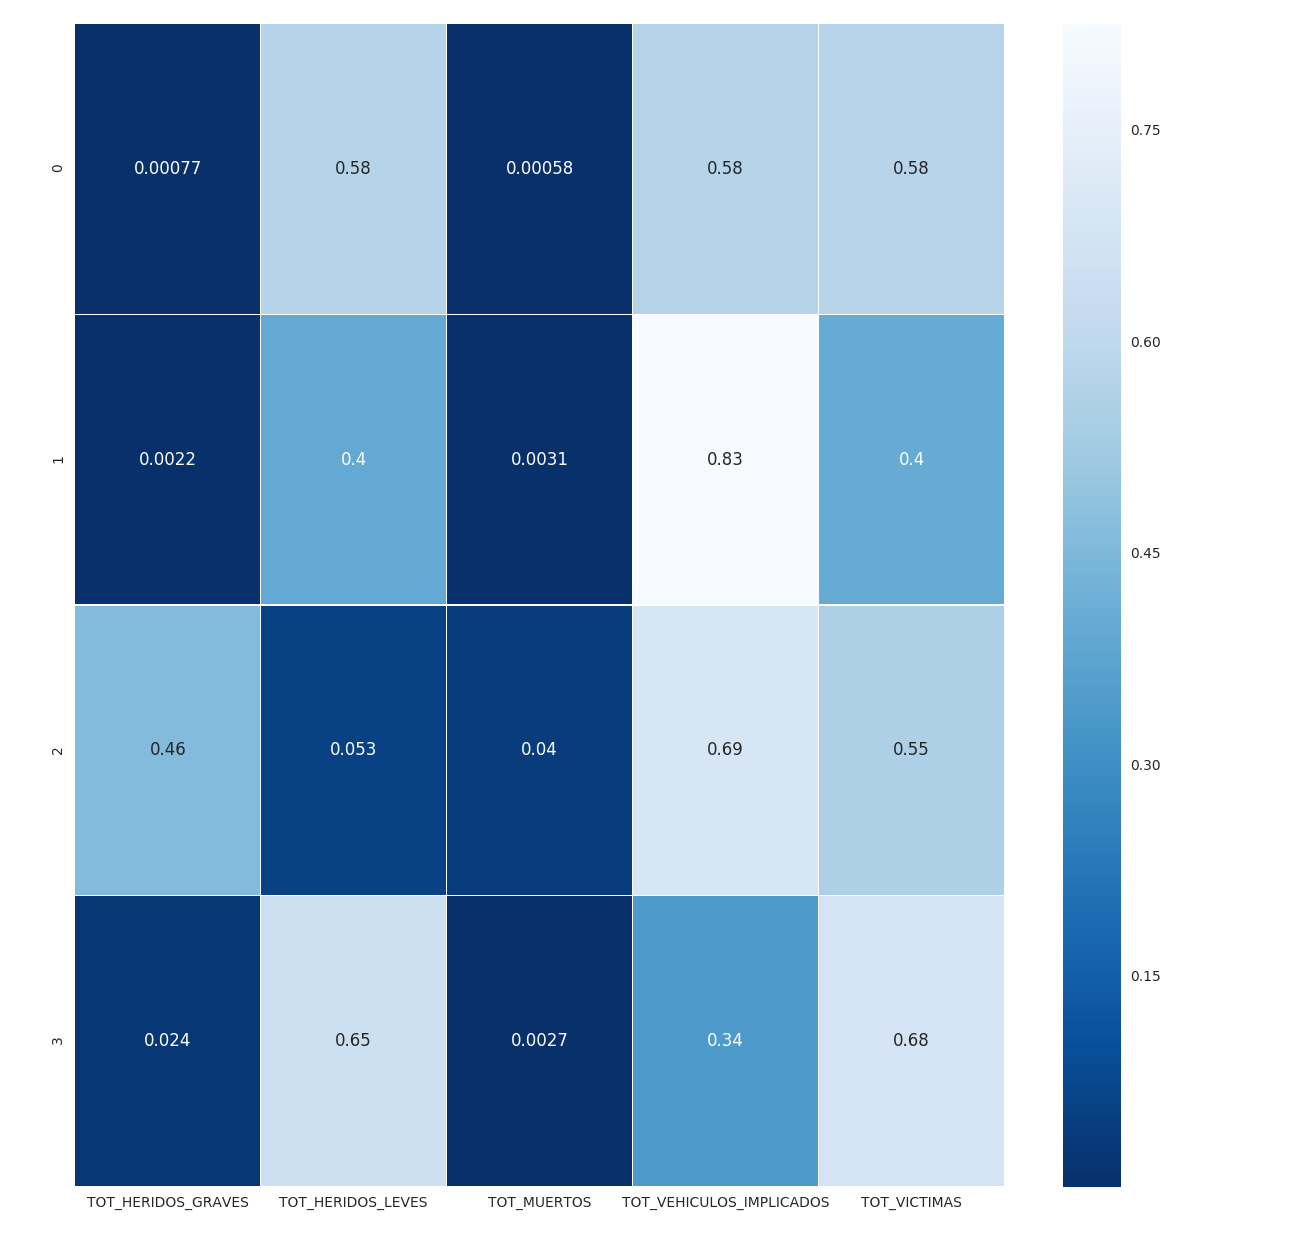
\includegraphics[scale=0.25]{../imagenes/heatmap_caso1_K-medias.png}
		\caption{Heatmap KMedias}
		\label{fig:hm_caso1_KMedias}
	\end{figure}

	\vspace{0.06in}

	Como se puede ver en el heatmap del algoritmos Agglomerative Clustering, hay clusters que no aparecen, esto es así porque se ha hecho un filtrado para eliminar aquellos clusters que tienen un número de elementos muy pequeño (por ejemplo un cluster de 3 elementos) ya que no son representativos de la muestra.
	
	\vspace{0.06in}
	
	Mirando el heatmap, podemos ver que existen algunos clusters para aquellos casos donde el número de muertos es elevado. También podemos ver que otros clusters clasifican aquellos accidentes donde el número de coches es mucho mayor pero el número de víctimas no es muy elevado.
	
	\vspace{0.06in}
	Si nos fijamos en el scatter matrix, podemos ver que cuanto mayor es el número de víctimas pero el número de heridos graves se mantiene hay 5 clusters diferentes, y que cuando el número de víctimas se mantiene pero el número de heridos graves aumenta solamente hay dos 2 clusters, cuando los dos aumentan hay 4 clusters diferentes. En relación con los heridos leves y el total de víctimas, existen diferentes clusters dependiendo del número de víctimas y el número de heridos. Por último, en relación entre el número de coches implicados y el número de víctimas hay 5 o 6 clusters.
	
	\vspace{0.06in}
	La columna del total de muertos no es muy informativa, ya que no se puede ver ninguna relación con las otras variables. La columna de total de heridos graves tampoco no aporta mucha información relevante para describir tipos de causas. Por último, la columna de total de heridos leves, al igual que el total de víctimas y el número de vehículos implicados, hay 7 u 8 clusters representados para representar los diferentes casos (pocos heridos, gran número de vehículos implicados, muchos heridos, pocos vehículos implicados, casos intermedios).
	
	\vspace{0.06in}
	Para el algorimto de K-medias la interpretación es más sencilla ya que contamos con menos clusters. El primero de los clusters representa accidentes donde hay relativamente pocos heridos leves y una gran cantidad de vehículos implicados. El segundo cluster representa accidentes con menos vehículos implicados pero más heridos leves. El tercer cluster representa accidentes con un gran número de heridos graves y bastantes vehículos implicados. Y por último el cuarto cluster representa accidentes con un gran número de heridos leves pero con pocos vehículos implicados.
	
	\vspace{0.06in}
	Como conclusión, podemos decir que dentro de las islas que hay en España los tipos de accidentes más comunes son accidentes normalmente con pocos heridos graves, suele haber más heridos leves, con un número de vehículos implicados variable; y accidentes con heridos graves que normalmente implican a pocos vehículos.
	
	
	\subsection[Caso de estudio 2]{Segundo caso de estudio: accidentes en Cataluña cada 30 días.}
	\subsubsection{Introducción.}
	Para este segundo caso de estudio seleccionaremos los accidentes sucedidos en Cataluña simplemente. Las variables que vamos a utilizar para el estudio son el total de víctimas en 30 días, el total de heridos graves en 30 días, el total de heridos leves en 30 días y el total de vehículos.
	
	\vspace{0.06in}
	
	El tamaño total del caso de estudio es de 23831 accidentes, aunque para el estudio utilizaremos solamente 15000 de ellos seleccionados de forma aleatoria utilizando una semilla para obtener siempre el mismo conjunto de datos. 
	
	\subsubsection{Parámetros de los algoritmos.}
	Para este caso de uso, se ha aumentado el número de clusters que utiliza el algoritmo K-medias, en vez de ser 4, a pasado a ser 6.
	Además, para el algoritmo de Mean Shift, a la hora de calcular el atributo \textit{bandwidth} se calcula con el parámetro \textit{quantile} igual a 0.3.
	
	\vspace{0.06in}
	Como último cambio realizado, se ha cambiado el número de clusters que debe calcular el algoritmo Agglomerative Clustering a 76 (MeanShift también calcula 76 clusters diferentes).
	\subsubsection{Resultados obtenidos.}
	
	\begin{table}[H]
	\centering
		\begin{tabular}{lrrrr}
			\toprule
			Name  &N clusters&	HC metric& 	SC metric& 	Time (s) \\
			\midrule  
			AC&       	76&        	1015216.69&	0.98&      	3.65 \\     
			Birch&     	12&        	3260.24&   	0.56&      	0.19 \\      
			MeanShift&  	76&        	134946.88& 	0.96&      	0.23 \\     
			SpectralC&  	6&         	38234.88&  	0.85&      	39.50 \\     
			K-medias&	6&         	42406.44&  	0.87&      	0.05\\      
			\bottomrule
		\end{tabular}
	\caption{Resultados algoritmos en el segundo caso de estudio}
	\label{table:res_caso2}
	\end{table}

	Para este caso se puede ver que el algoritmo de K-medias mejora los resultados que obtenía en el caso de estudio anterior. El algoritmo Birch, sin embargo, obtiene unos resultados bastante pobres en comparación con le resto de algoritmos. Utilizaremos estos dos algoritmos para compararlos e intentar entender como clasifica los datos cada uno de ellos. Aunque la conclusión final se hará con las gráficas aportadas por el algoritmo K-Medias dado que sus métricas son muchos mejores que las del Birch. 
	\subsubsection{Interpretación de la segmentación.}
	
	\begin{figure}[H]
		\centering
		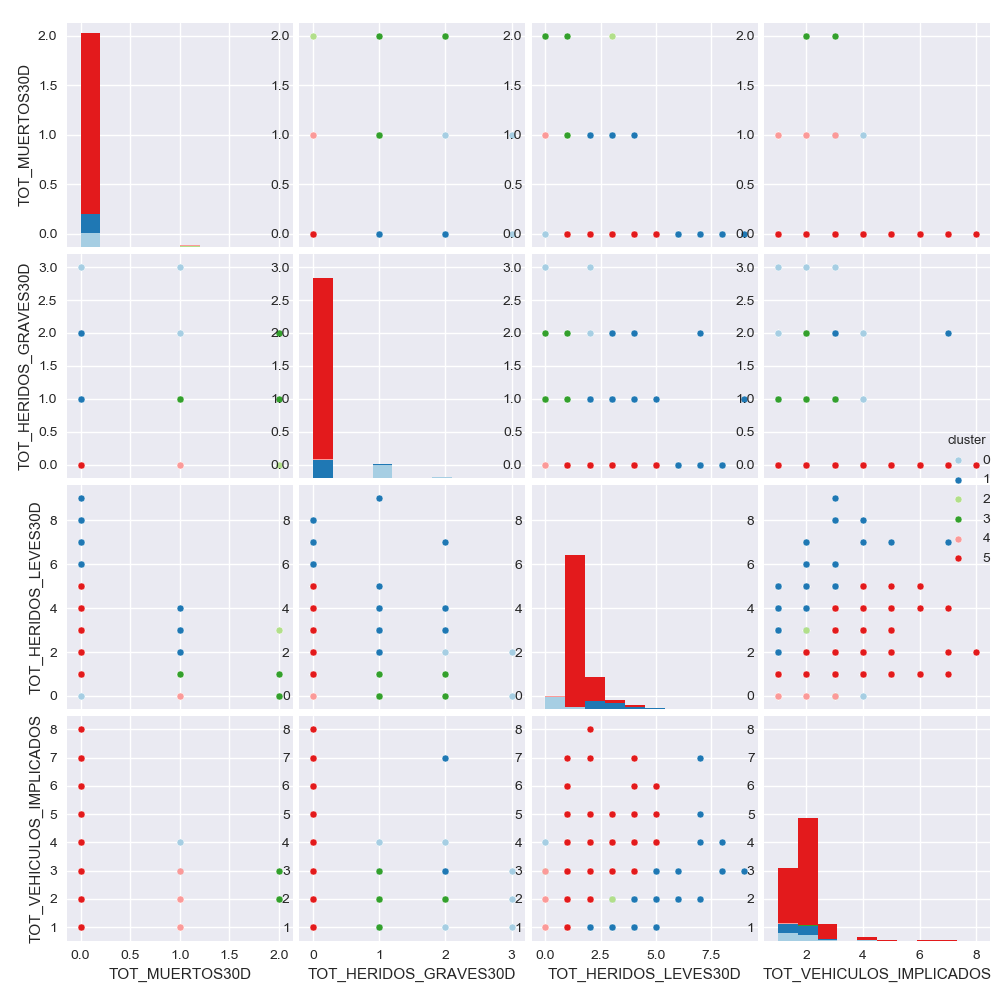
\includegraphics[scale=0.25]{../imagenes/scatterMatrix_caso2_Birch.png}
		\caption{Scatter Matrix Birch}
		\label{fig:scatter_caso2_Birch}
	\end{figure}
	
	\begin{figure}[H]
		\centering
		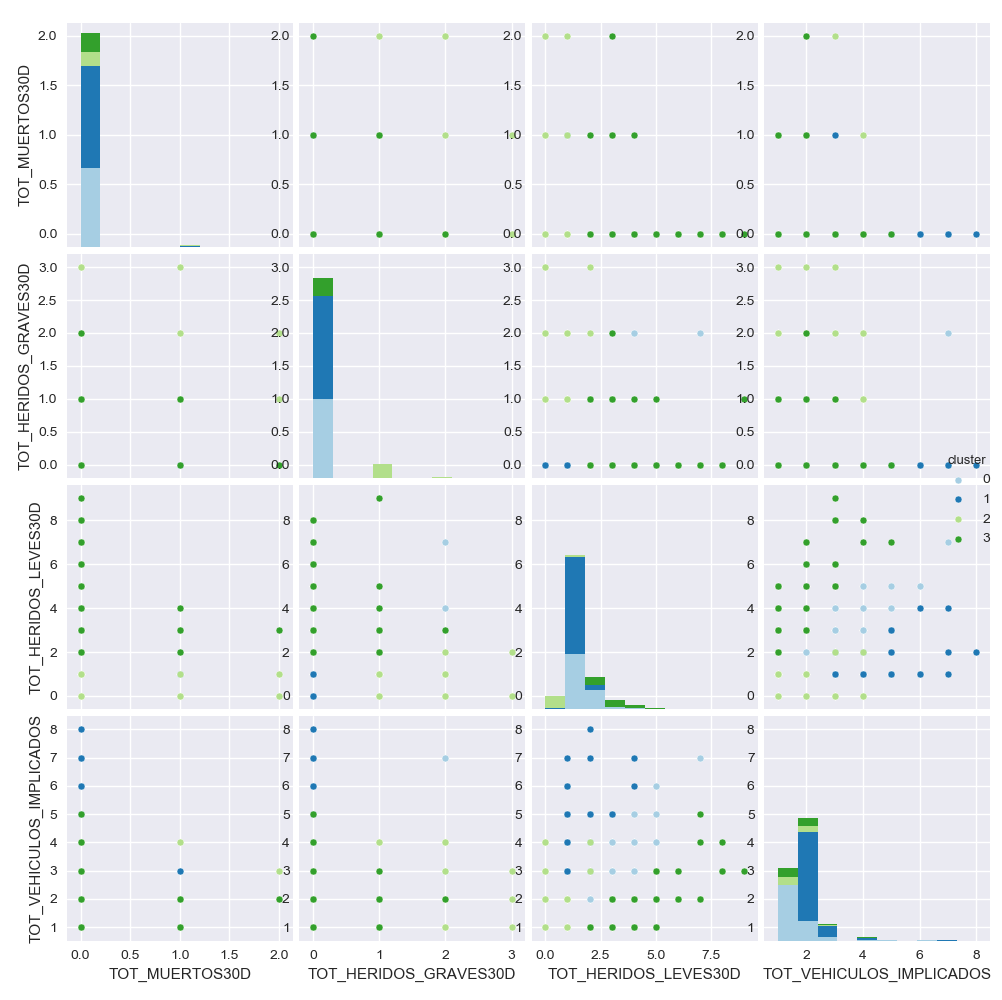
\includegraphics[scale=0.25]{../imagenes/scatterMatrix_caso2_K-medias.png}
		\caption{Scatter Matrix KMedias}
		\label{fig:scatter_caso2_KMedias}
	\end{figure}
	
	\begin{figure}[H]
		\centering
		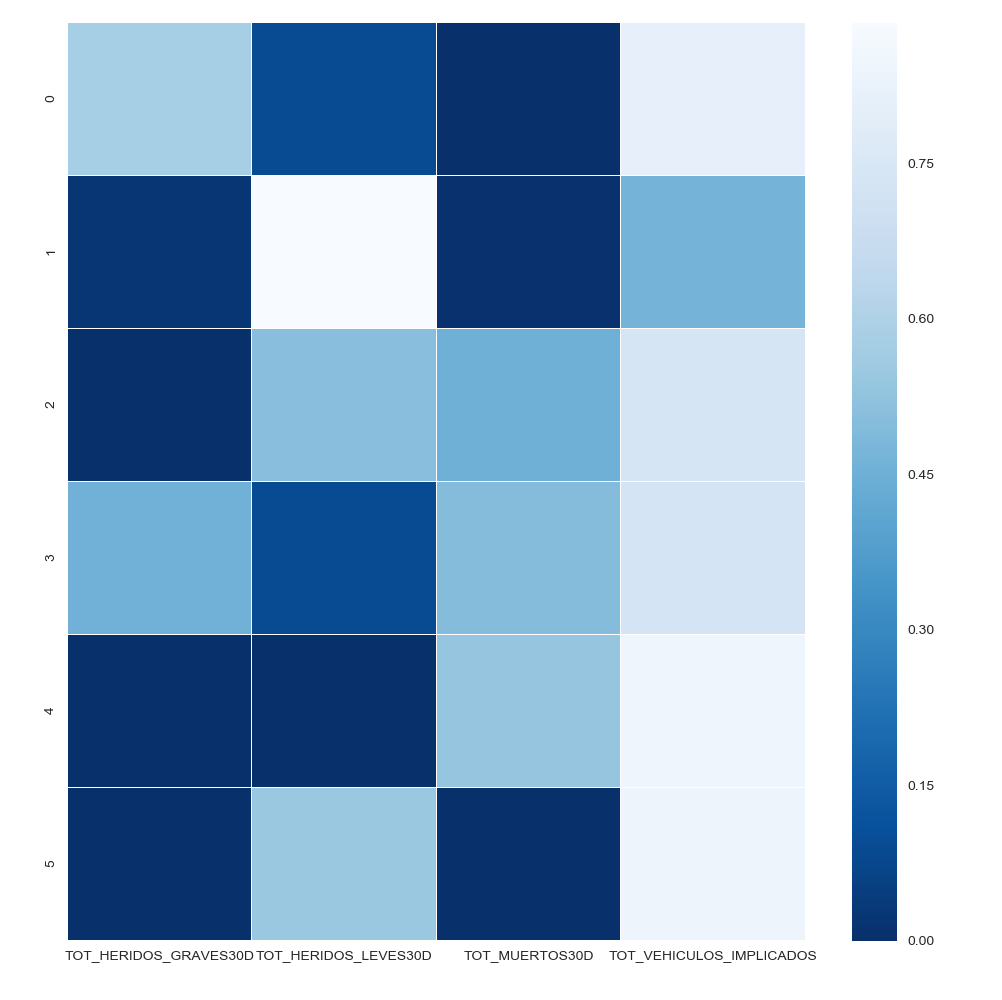
\includegraphics[scale=0.3]{../imagenes/heatmap_caso2_Birch.png}
		\caption{Heatmap Birch}
		\label{fig:hm_caso2_Birch}
	\end{figure}
	
	\begin{figure}[H]
		\centering
		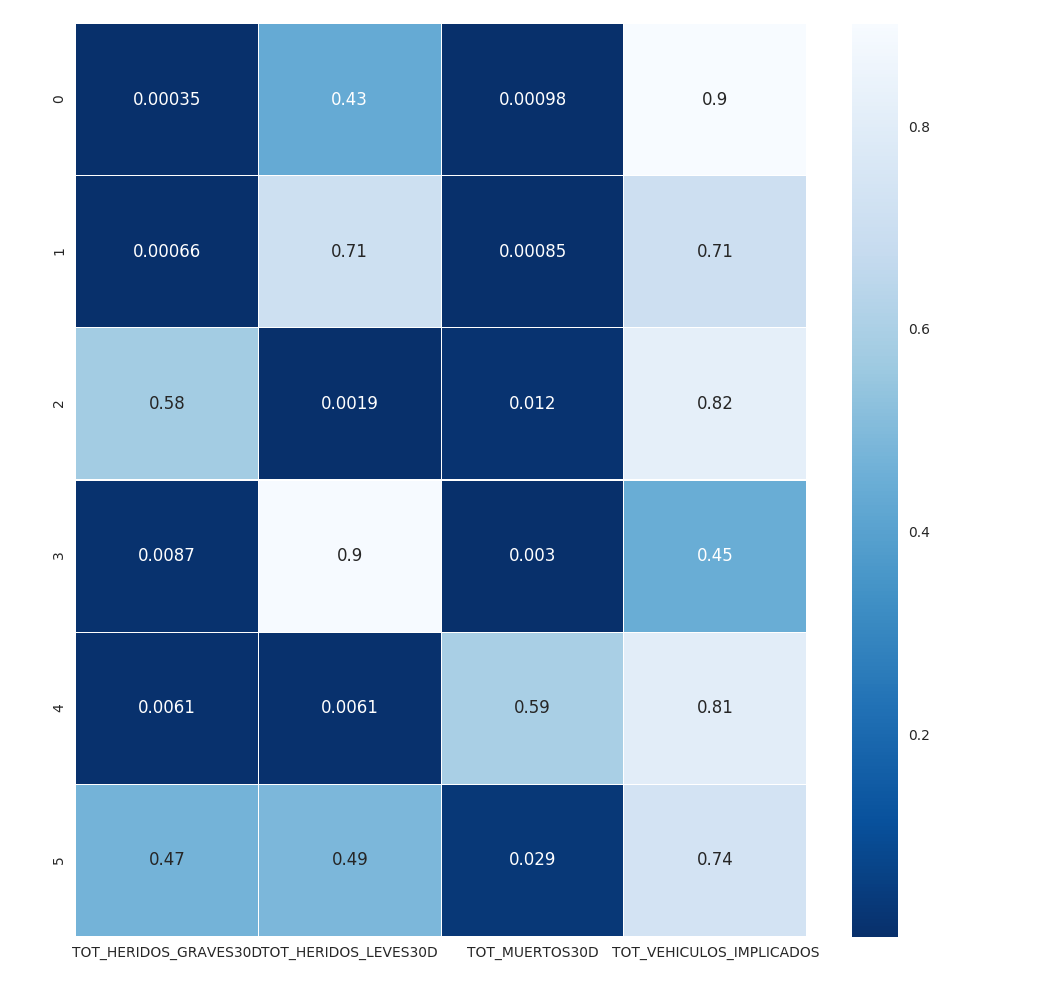
\includegraphics[scale=0.3]{../imagenes/heatmap_caso2_K-medias.png}
		\caption{Heatmap KMedias}
		\label{fig:hm_caso2_KMedias}
	\end{figure}

	\vspace{0.06in}
	Como se puede ver el scatter matrix, el cluster 11 ocupa la gran mayoría una gran parte de los datos, los cuáles cuentan con al menos 2 ó más heridos leves, hay pocos heridos graves y pocos muertos. El otro cluster mayoritario es el cluster 7, que representa aquellos accidentes para los cuales se hay un número mayor de coches implicados.
	
	\vspace{0.06in}
	
	Para este caso, no merece la pena mirar el heatmap de este algoritmo, ya que al haber tantos grupos con pocos elementos las medias no representan bien los clusters.
	
	\vspace{0.06in}
	
	Para el algoritmo de K-Medias, podemos ver si miramos el heatmap que el primer cluster representa accidentes con un número alto de heridos leves y un número alto de vehículos implicados. El segundo cluster representa accidentes con menos heridos leves que en el primer cluster pero con más vehículos implicados en el accidente. El tercero representa accidente con muchísimos heridos leves. El cuarto representa accidentes dónde ha habido muertos y una gran cantidad de vehículos implicados. El quinto representa accidentes con un heridos graves y gran cantidad de vehículos implicados. Por último, el sexto representa accidentes donde hay la misma cantidad de heridos graves que de heridos graves y una cantidad alta de vehículos implicados.
	
	\vspace{0.06in}
	
	Si miramos el scatter matrix, podemos ver que lo que indica el heatmap también se corresponde con la información del scatter matrix.
	
	\vspace{0.06in}

	\subsection[Caso de estudio 3]{Tercer caso de estudio: accidentes en Bizkaia cuando llueve}
	\subsubsection{Introducción.}
	Para el tercer caso de estudios he seleccionado los accidentes en Bizkaia en los cuales había lluvia.
	
	\vspace{0.06in}
	Las variables que se van a utilizar para este caso de estudio son las misma que en el primer caso de estudio. El tamaño de la muestra es 1724, por lo que estudiaremos el conjunto de datos en su totalidad para el estudio.
	
	\subsubsection{Parámetros de los algoritmos.}
	Para este algoritmo, se ha cambiado el número de clusters a 5 para el K-Medias ya que con está alcanzaba mejores resultados. Para el algoritmo de Mean Shift se ha cambiado el parámetro con el que se calcula el \textit{bandwidth} \textit{quantile} a 0.4. El algoritmo Spectral Clustering calcula 4 clusters, el algoritmo Birch calcula 5 y el algoritmo Agglomerative Clustering utiliza 26 clusters (algunos de estos se eliminarán después si son muy pequeños).
	\subsubsection{Resultados obtenidos.}
	\begin{table}[H]
	\centering
		\begin{tabular}{lrrrr}
			\toprule
			Name&       	N clusters&	HC metric& 	SC metric& 	Time (s) \\  
			Birch&        	5&         	1726.42&   	0.82      	0.02 \\      
			MeanShift&      	16&        	3461.24&   	0.87&      	0.03 \\     
			SpectralC&      	4&         	2315.11&   	0.82&      	0.26 \\      
			K-medias&       	6&         	4844.23&   	0.90&      	0.01 \\      
			AC&             	26&        	31680.00&  	0.96&      	0.04 \\      
			\bottomrule
		\end{tabular}
	\caption{Resultados algoritmos en el tercer caso de estudio}
	\label{table:res_caso3}
	\end{table}

	\vspace{0.06in}
	Como se puede ver en la tabla, el algoritmo Agglomerative Clustering es el que mejores resultados obtiene, por detras está el algoritmo K-Medias, y después el algoritmo Mean Shift.
	
	\vspace{0.06in}
	Para este caso de estudio, se analizarán las gráficas generadas para los algoritmos de Agglomerative Clustering y Mean Shift.

	\subsubsection{Interpretación de la segementación.}
	
	Lo primero que vamos a hacer es generar un dendograma de la jerarquía de clusters que se obtiene del algoritmo Agglomerative Clustering.
	
	\begin{figure}[H]
		\centering
		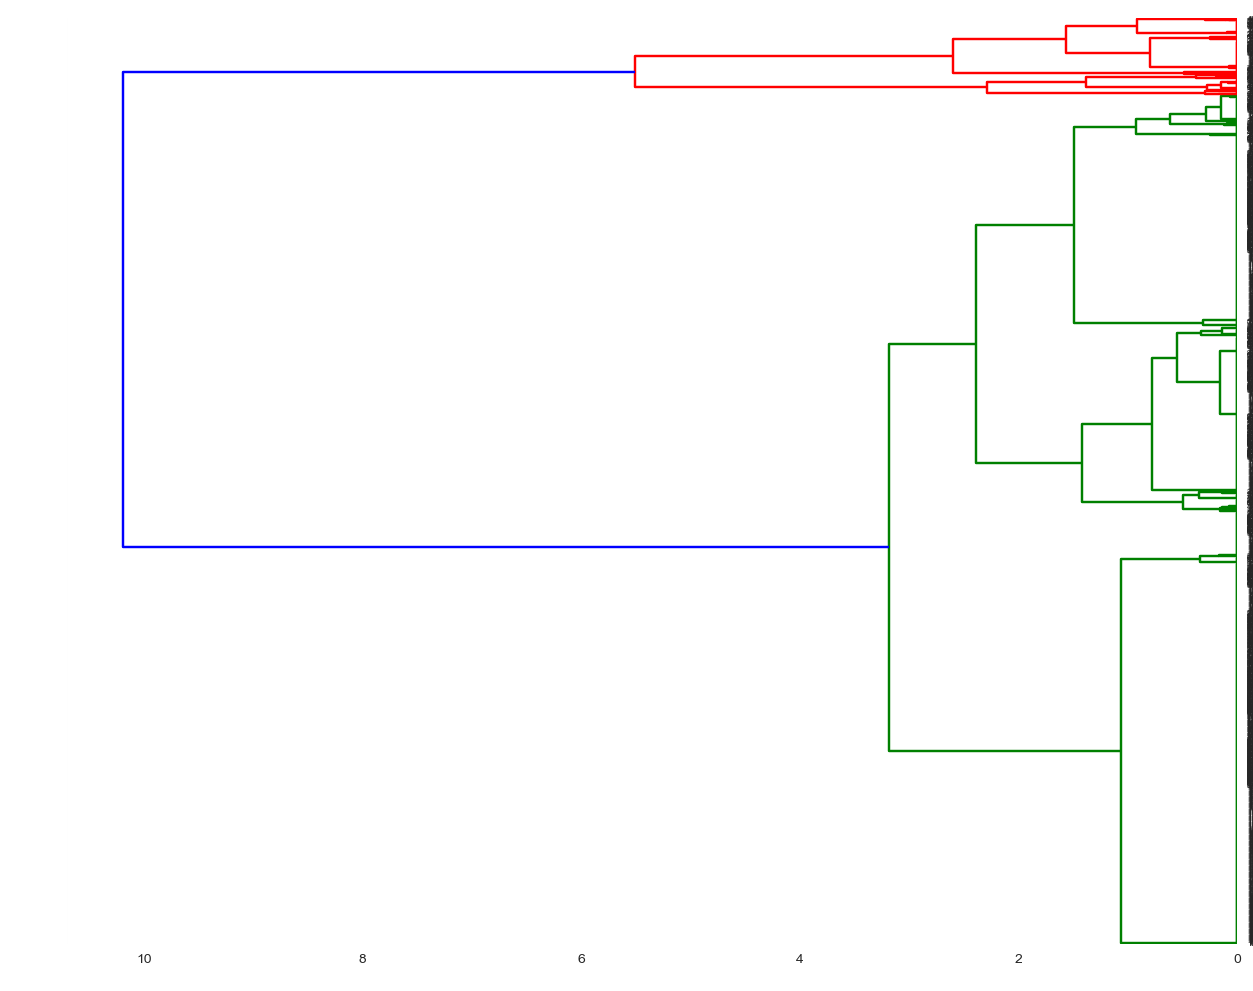
\includegraphics[scale=0.25]{../imagenes/dendograma_AC.png}
		\caption{Dendograma Agglomerative Clustering}
		\label{fig:dendogram_caso3_AC}
	\end{figure}

	\vspace{0.06in}
	Como se puede ver en el dendograma, existe una gran cantidad de clusters que no representan muchos datos, por desgracia, no podemos saber cuáles son porque se borran las letras de la izquierda.
	
	\begin{figure}[H]
		\centering
		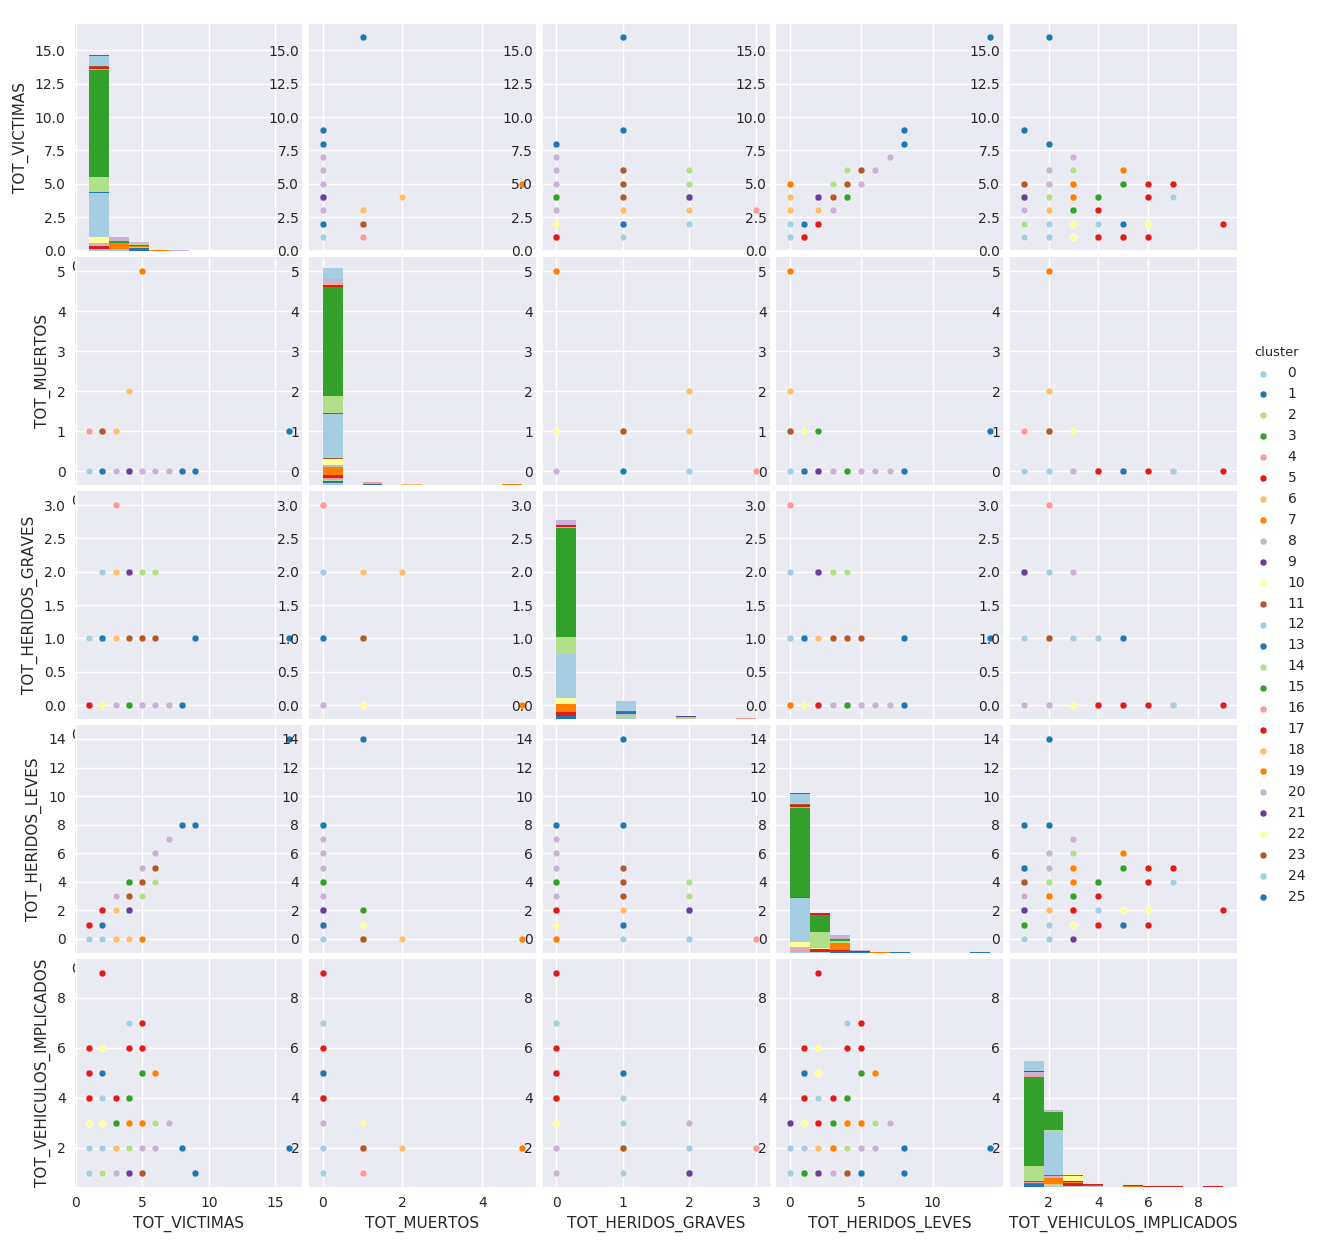
\includegraphics[scale=0.25]{../imagenes/scatterMatrix_caso3_AC.png}
		\caption{Scatter Matrix Agglomerative Clustering}
		\label{fig:scatter_caso3_AC}
	\end{figure}
	
	\begin{figure}[H]
		\centering
		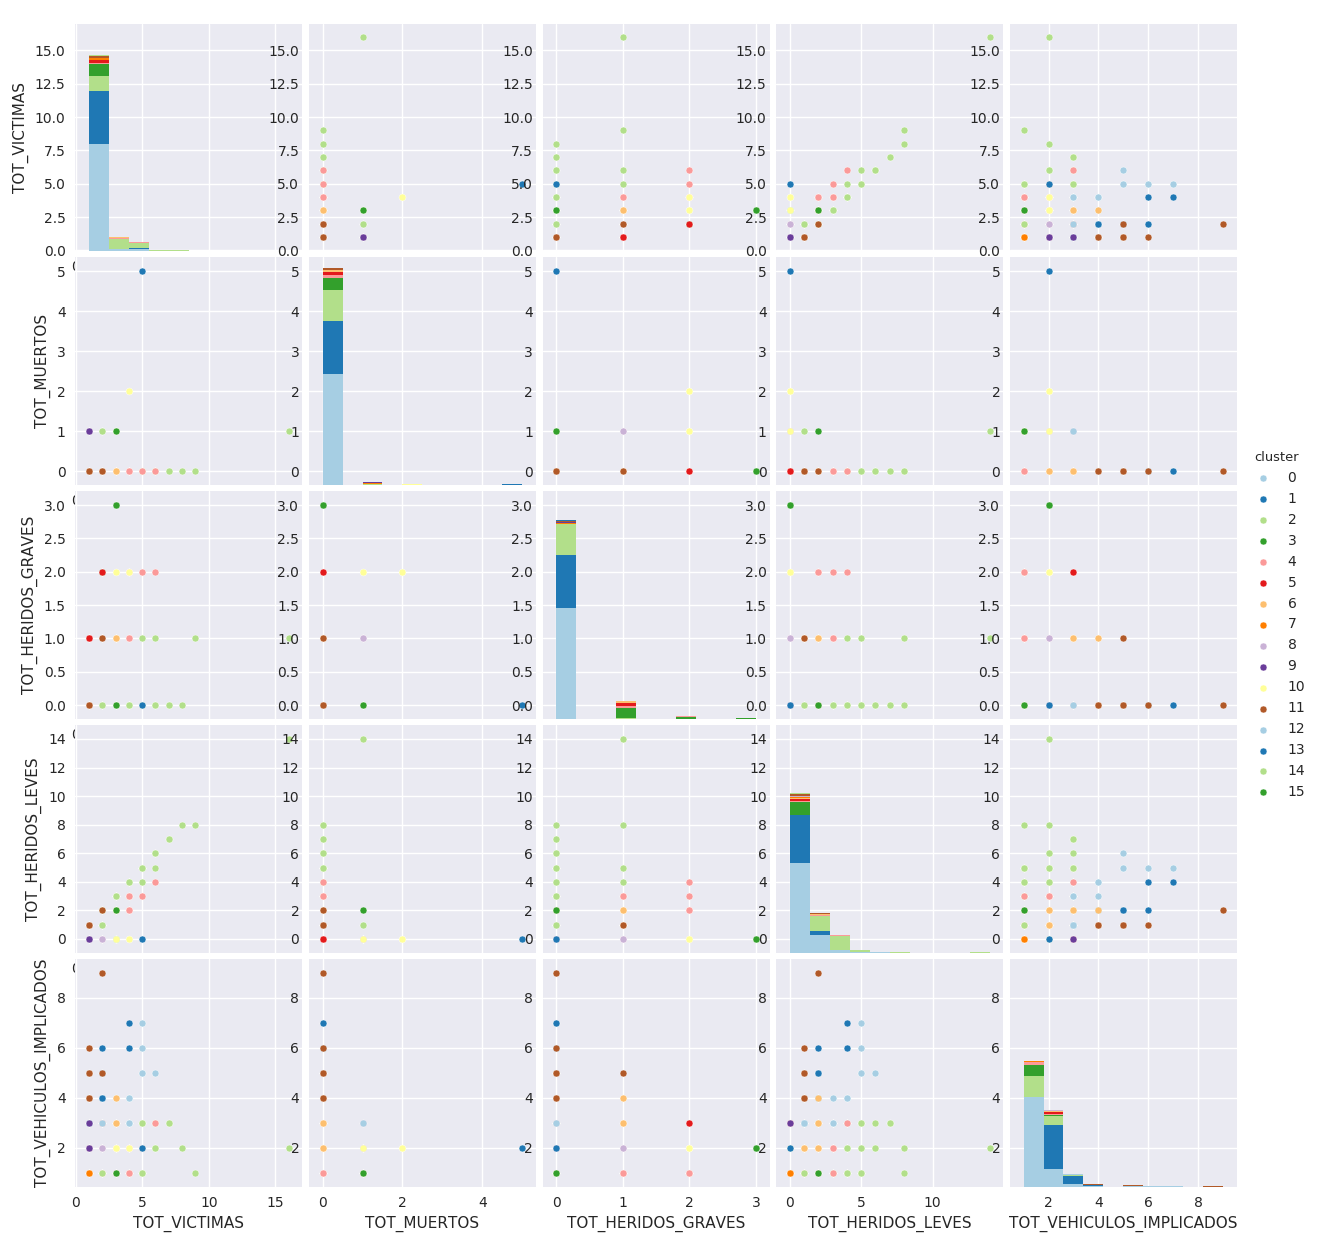
\includegraphics[scale=0.25]{../imagenes/scatterMatrix_caso3_MeanShift.png}
		\caption{Scatter Matrix MeanShift}
		\label{fig:scatter_caso3_MS}
	\end{figure}
	
	\begin{figure}[H]
		\centering
		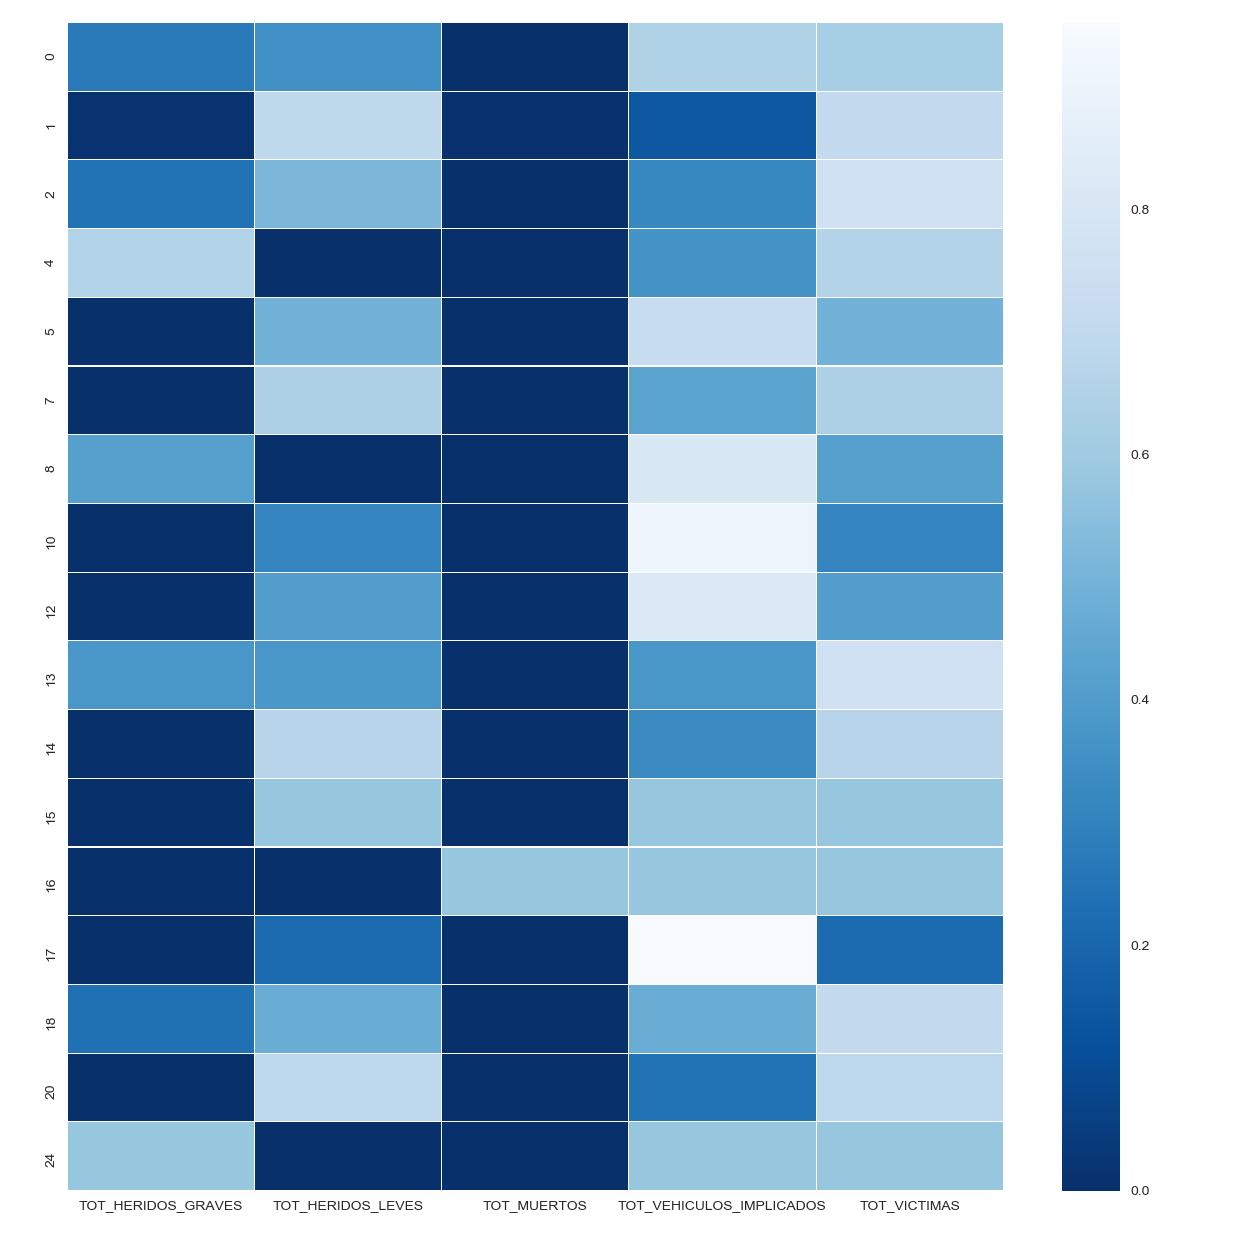
\includegraphics[scale=0.25]{../imagenes/heatmap_caso3_AC.png}
		\caption{Heatmap Agglomerative Clustering}
		\label{fig:hm_caso3_AC}
	\end{figure}
	
	\begin{figure}[H]
		\centering
		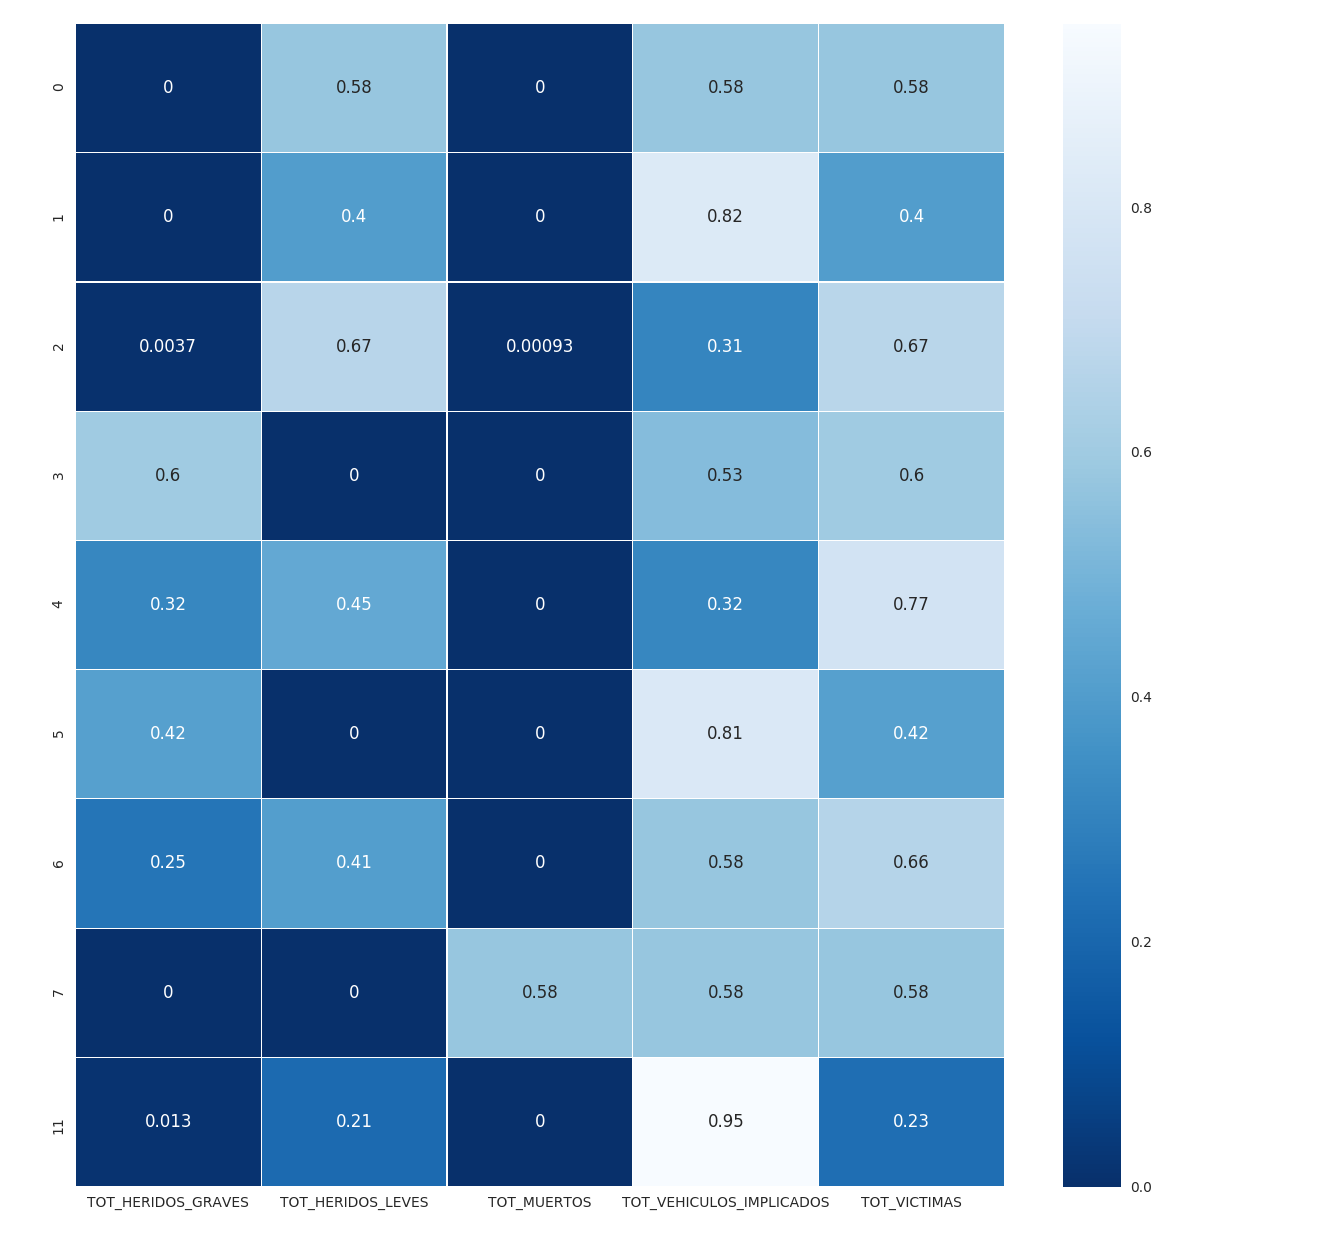
\includegraphics[scale=0.25]{../imagenes/heatmap_caso3_MeanShift.png}
		\caption{Heatmap Mean Shift}
		\label{fig:hm_caso3_MS}
	\end{figure}

	\vspace{0.06in}
	Como se puede ver en el heatmap del algoritmo Agglomerative Clustering, se han eliminado algunos clusters por representar muy pocos datos. Además, podemos reconocer 3 clusters que tienen un número de heridos graves alto y no hay heridos leves, mientras que se diferencian sobre todo en el número de vehículos implicados en los accidentes. También se puede ver que la columna de total de muertos es 0 o casi 0 en todos los clusters, por lo cuál podríamos quitarla ya que no nos está aportando nada al estudio.
	
	\vspace{0.06in}
	Si miramos el scatter matrix, podemos ver que existe una relación directa entre víctimas y heridos leves, sin embargo, no es así con los heridos graves ya que hay muchos menos heridos graves que leves dentro del conjunto de datos, por ello, se utilizan diferentes clusters para cuando hay 1,2 ó 3 heridos graves. El número de vehículos implicados en los accidentes también se relaciona de forma relativamente directa con el número de víctimas y con el número de heridos leves; para el caso de los heridos graves, se puede el número de vehículos implicados disminuye cuando aumenta el número de heridos.
	
	\vspace{0.06in}
	
	Para el algoritmo Mean Shift, también se puede ver que algunos clusters se han eliminado por falta de elementos. Al igual que en el algoritmo anterior, existe un relación directa entre número de víctimas y número de heridos leves, también se puede ver que la columna de total de muertos solo hay un cluster (7) que lo represente.
	
	\vspace{0.06in}
	Como resultado, podemos concluir que los accidentes que hay en bizkaia cuando hay lluvia suelen que implican heridos graves suelen implicar bastantes coches, pero en cambio aquellos que implican heridos leves no tiene porque implicar un número alto de vehículos implicados. Por último, en los accidentes donde hay un número alto de heridos graves suele haber un número parecido de heridos leves y no implica muchos vehículos.

	\section[Contenido adicional]{Contenido adicional}
	\section[Bibliografía]{Bibliografía.}
	\bibliography{citas} %archivo citas.bib que contiene las entradas 
	\bibliographystyle{IEEEtran} % hay varias formas de citar


\end{document}